
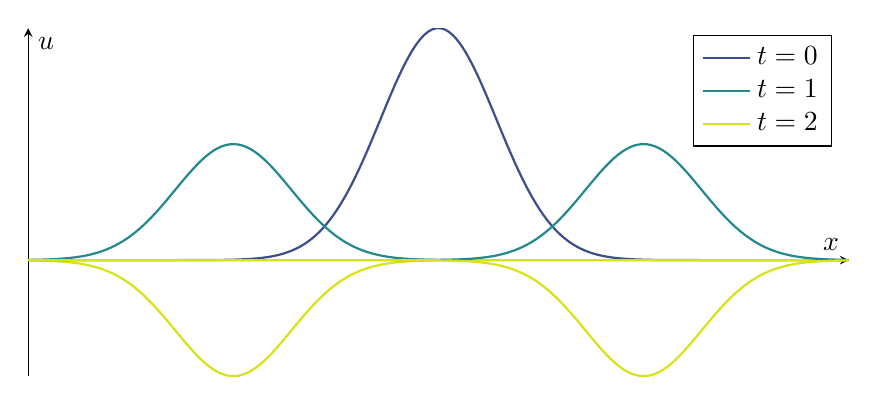
\begin{tikzpicture}
\begin{axis}[domain = 0:1, colormap/viridis, cycle list={[indices of colormap = {0, 4, 8, 12, 16} of viridis]}, width = 12cm, height = 6cm, axis lines = middle, ticks = none, xlabel = $x$, ylabel=$u$]
\addplot +[mark = none, samples=200, thick, index of colormap = 4] {0.1 * e^(-(10 * (x - 0.5))^2)};
\addplot +[mark = none, samples=200, thick, index of colormap = 8] {0.05 * e^(-(10 * (x - 0.25))^2)};
\addplot +[mark = none, samples=200, thick, index of colormap = 16] {-0.05 * e^(-(10 * (x - 0.25))^2)};
\addplot +[mark = none, samples=200, thick, index of colormap = 8] {0.05 * e^(-(10 * (x - 0.75))^2)};
\addplot +[mark = none, samples=200, thick, index of colormap = 16] {-0.05 * e^(-(10 * (x - 0.75))^2)};
\addlegendentry{$t = 0$}
\addlegendentry{$t = 1$}
\addlegendentry{$t = 2$}
\end{axis}
\end{tikzpicture}
